\documentclass{article}
\usepackage[utf8]{inputenc}
\usepackage{graphicx}
\usepackage[margin=2.5cm]{geometry}
\usepackage{eso-pic}
\usepackage{hyperref}
\usepackage{wrapfig}
\usepackage{array}
\usepackage{enumitem}
\AddToShipoutPictureBG{%
    \AtPageLowerLeft{
        % \hspace{1cm}
        
\includegraphics[width=4.5cm]{img/Java-Hutts2.png}
    }
}
\title{Testing Report}
\date{2017}
\def \project{Electronic ID Verification }
\begin{document}

\makeatletter
    \begin{titlepage}
        \begin{center}
            
\includegraphics[width=0.7\linewidth]{img/up.png}\\[4ex]
            {\huge \bfseries \@title }\\[2ex]
            {\LARGE \textbf{Team:} Java the Hutts}\\[2ex]
            {\LARGE \@date}\\[2ex]
            {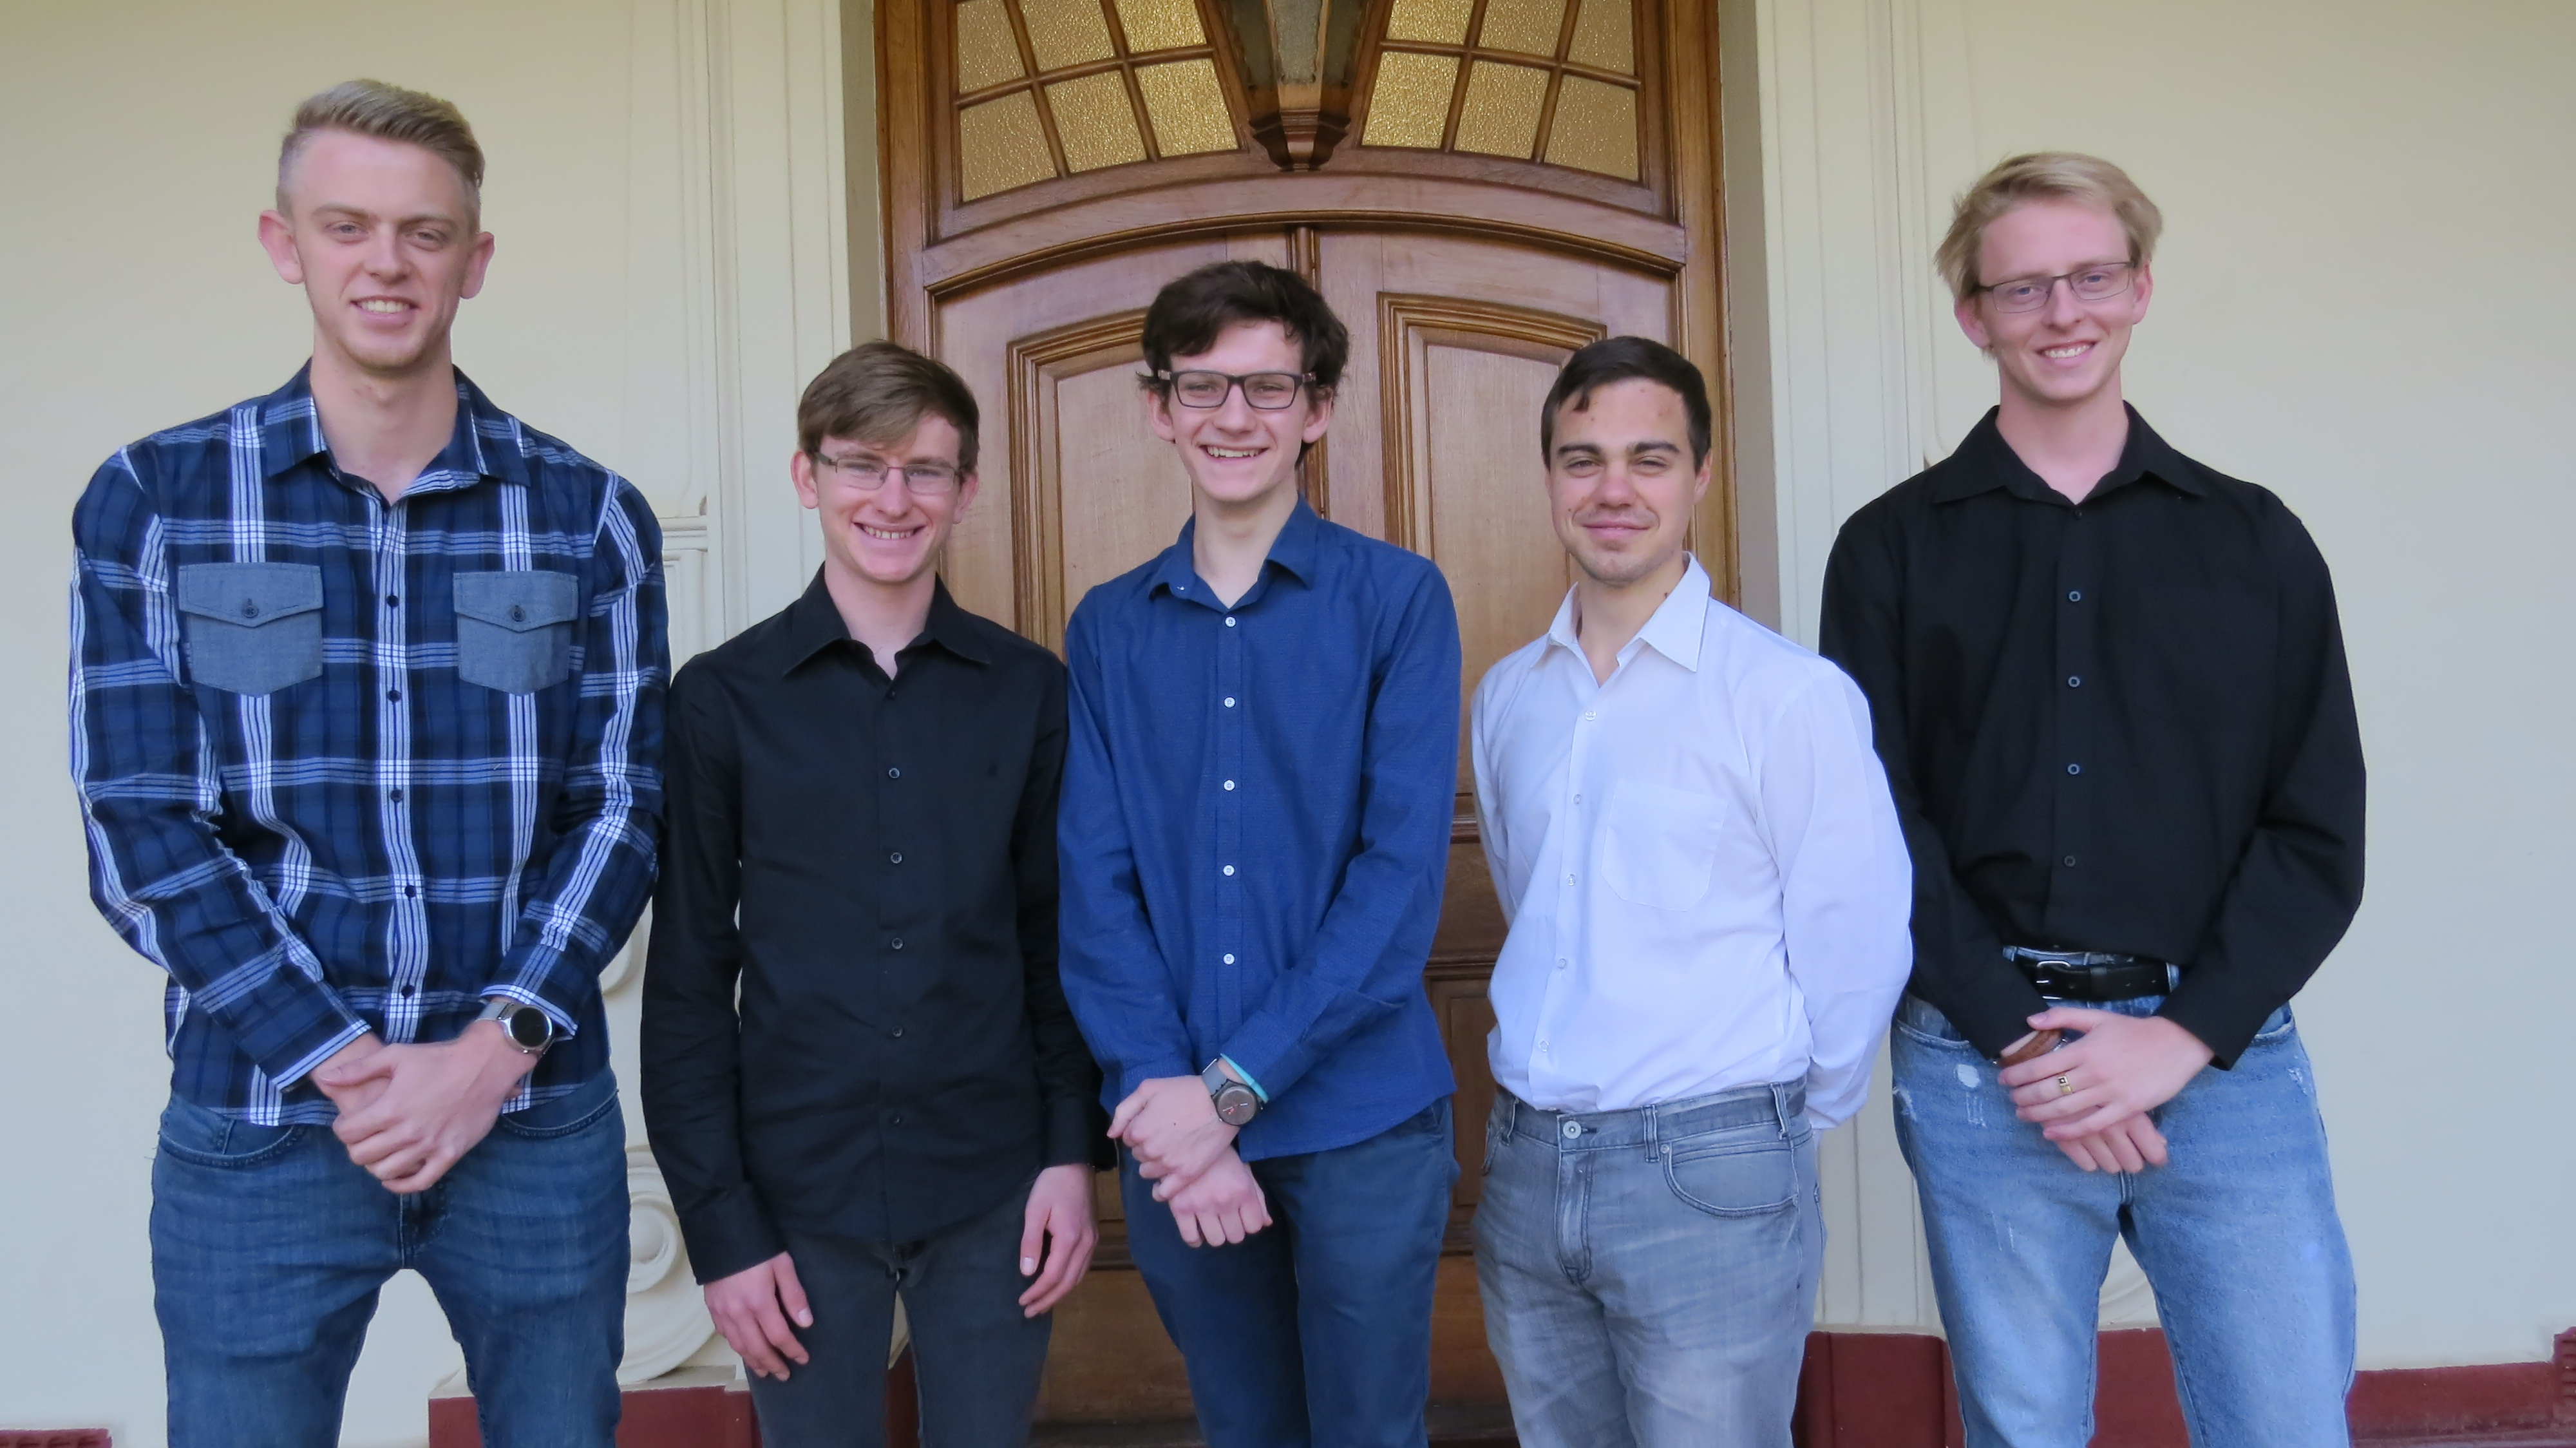
\includegraphics[width=\linewidth]{img/team_photo.jpg}}\\[2ex]
            {\large  Nicolai van Niekerk\\ \texttt{nicvaniek@gmail.com}}\\[2ex]
            {\large  Marno Hermann\\ \texttt{marno@barnton-consulting.co.za}}\\[2ex]
            {\large  Stephan Nell\\ \texttt{nellstephanj@gmail.com}}\\[2ex]
            {\large  Jan-Justin van Tonder\\ \texttt{J.vanTonder@tuks.co.za}}\\[2ex]
            {\large  Andreas Nel\\ \texttt{nel.andreas1@gmail.com}}\\[2ex]
        \end{center}
        
    \end{titlepage}
\makeatother

\cleardoublepage
\thispagestyle{empty}
\tableofcontents
\newpage

\setcounter{page}{1}
	\section{Overview}\label{sec:intro}
		This document serves to present the testing coverage report of the \project project thus far, including branch coverage and overall test coverage.
		\subsection{Testing Status, Technologies Used and Testing Methods}
		As the project currently stands, the more in-depth testing is performed on the text manager, which is used to extract text from an ID document, due to the fact that this is the most crucial subsystem of the entire project. We make use of the black-box testing method as the project currently stands, but are in the process of also integrating white-box testing. Tests are written using the \textit{pytest} library for the Python programming language, and all unit tests and integration tests are run automatically by our build tool, \textit{PyBuilder}. Our code coverage and branch coverage is measured automatically via the \textit{coverage} plugin for PyBuilder - where a branch refers to a single instance of execution of the program (each conditional statement in the code increases the amount of branches).
		
		Note that some of the files referenced in the report indicate that there are 0 (zero) statements in the code. This is due to the fact that these files are required in order to mark certain parts of code as modules or packages, and that extra functionality has yet to be implemented in these files.
	\section{Report}
	\begin{figure}[h]
		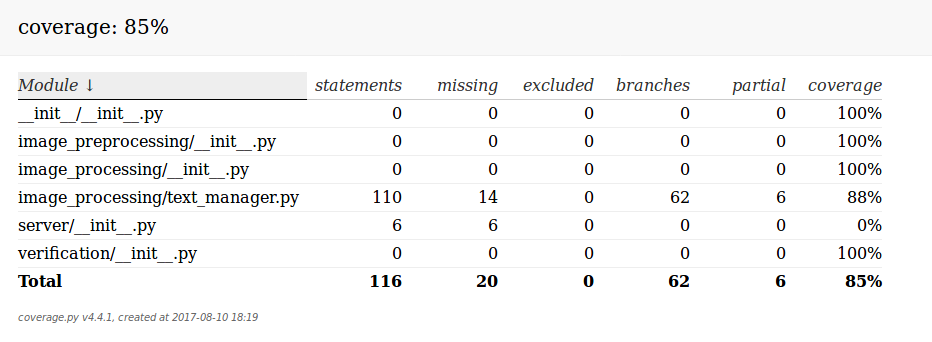
\includegraphics[scale=0.5]{img/coverage.png}
		\caption{Test Report}
	\end{figure}
\end{document}
